\chapter{Results Analysis}



	In Reinforcement Learning, results vary a lot depending on the parameters of the training. To understand how we are going to compare the different algorithms, we have to first define some metrics. In this case, the metrics are:
	
	\begin{itemize}
		\item[\textendash]\textbf{The number of pick actions per episode}: When the agent performs a pick action and picks an object, the episode is ended. So, in this case, \textbf{the lowest the better}.
		\item[\textendash]\textbf{Reward per episode}: In each episode, the agent is trying to maximize the total reward, so, in this case, \textbf{the highest the better}
		\item[\textendash]\textbf{Number of steps per episode:} We want to minimize the time between picks. \textbf{The lower the better}
		\item[\textendash]\textbf{Evolution of successful episodes during the training:} As we already know, the episodes can be ended  because the agent has pick an object (success) or when the robot has reached the environment limits (not success). The number of unsuccessful episodes should decrease during the training.
		\item[\textendash]\textbf{Random actions per episode:} This is not actually a measure of performance but a measure of control. If the training is going well, when the number of random actions decreases, the rest of the measures should improve.
	\end{itemize}

	Once that we have the measures, we should understand how to compare this information. For example I have decided that, for the first 3 measures, we shouldn't take into account the information of unsuccessful episodes, because that could result on a false sense of improvement. Let's imagine the "Number of steps per episode" metric, if we took into account the non successful episodes, we could have an episodes of one steps thinking that we are improving, while we are actually worsen. The same could happen with the number of picks and even with the reward metric, because, although the reward for reaching the environment limits is really low, the reward of a failed pick is as low as the other, so we could also be having a false sense of improving.
	
	On the other hand, in order to have softer and more readable graphs, I have decided to plot the mean of the last N values instead of the values themselves. I probably got inspiration from the "Theory of Communications" course.
	
	The results gotten can be seen in the following set of figures. In \autoref{fig:picksperepisode} we can see how the pick actions per episode decreased during the training. The mean was between 1.2 and 1.4 which are goods results having in mind that we are only showing the successful episodes. The optimal value of this metric would be 1 pick per successful episode, so this results shows that there are much more successful picks than unsuccessful.
	
	\begin{figure}[H]
		\centering
		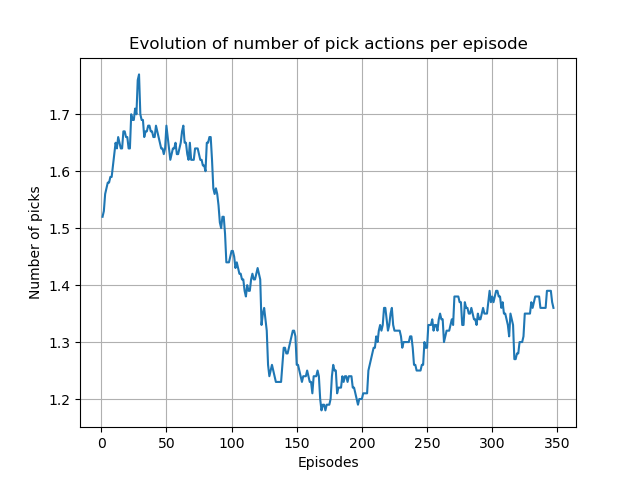
\includegraphics[width=0.7\linewidth]{Images/original_algorithm/picks_per_episode}
		\caption[Pick actions per episode]{Evolution of pick actions in episodes}
		\label{fig:picksperepisode}
	\end{figure}

	In \autoref{fig:rewardperepisode}, we can see how rewards evolve during the training. As we can see, the reward is increasing during the whole training. The reward is still negative but it is normal, because all the actions have negative rewards but the successful pick action, that has a positive reward.The objective of the training would be having positive rewards, that would mean picking a piece in the first 10 steps of the episode without failing any other pick. This is a performance that, unfortunately is still far from happening, although our performance is good enough to reach our objectives, as we will see later.
	
	\begin{figure}[H]
		\centering
		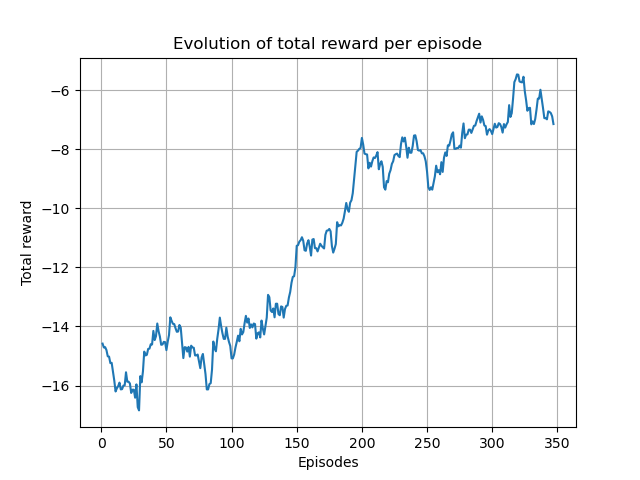
\includegraphics[width=0.7\linewidth]{Images/original_algorithm/reward_per_episode}
		\caption[Reward per episode]{Evolution of rewards through episodes}
		\label{fig:rewardperepisode}
	\end{figure}

	In \autoref{fig:stepsperepisode}, we can see the evolution of steps per episode. This metric has improve a lot, as we can see that the agent is picking pieces much faster than in the beginning.
	
	\begin{figure}[H]
		\centering
		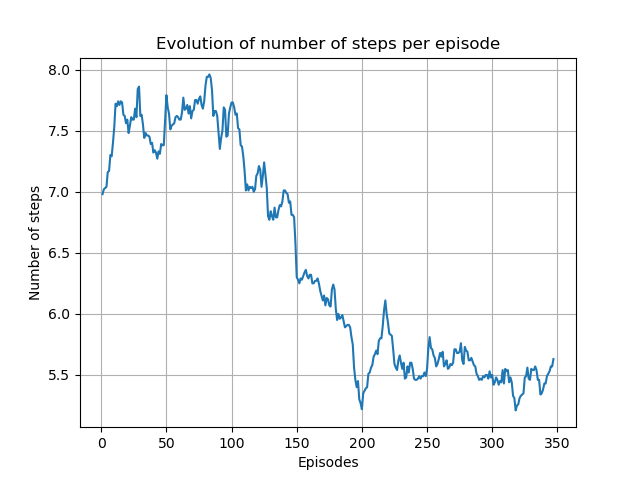
\includegraphics[width=0.7\linewidth]{Images/original_algorithm/steps_per_episode}
		\caption[Steps per episode]{Evolution of steps through episodes}
		\label{fig:stepsperepisode}
	\end{figure}

	As we said before, the improvement in the other metrics is important, but we have to check if this is happening when we reduce the number of random actions. If it doesn't, it can just be coincidence. In \autoref{fig:randomactions} we can see how the random actions kept decreasing during the training, showing that the good impressions of the training are well founded.
	
	\begin{figure}[H]
		\centering
		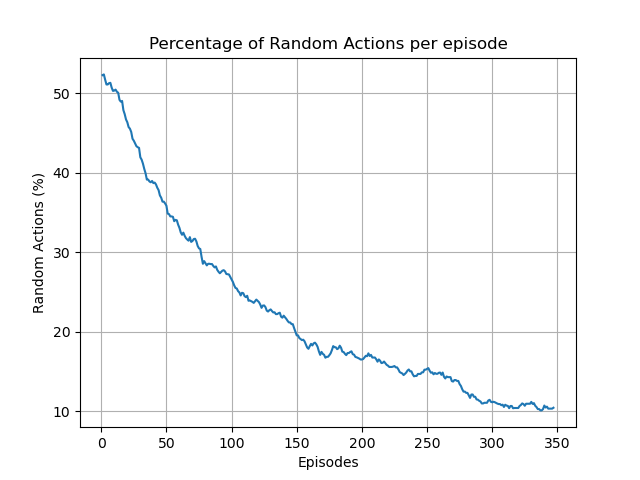
\includegraphics[width=0.7\linewidth]{Images/original_algorithm/random_actions}
		\caption[Random actions per episodes]{Evolution of random actions per episode}
		\label{fig:randomactions}
	\end{figure}


	Until now, all the news regarding were good. However, we cannot be completely happy with the results showed in \autoref{fig:successfulepisode}. In this image we can see how successful and non successful episodes have evolved during training. Having in mind that the big white holes (set of unsuccessful episodes) can be considered as accidents during the training (forgetting to re-fill the box with pieces, or failures of the system while calculating the robot coordinates), it seems like the rate of successful vs unsuccessful episodes improve over the training.
	
	However, This is probably the worst metric in the training, and it is something to improve in the next iterations. If I had to say the reason, I would say that sometimes, when the box is partially empty, the agent sees reaching the environment limits as a tool for picking a piece, because every time that the robot reaches the limits, the optimal point of starting is calculated.
	
	\begin{figure}
		\centering
		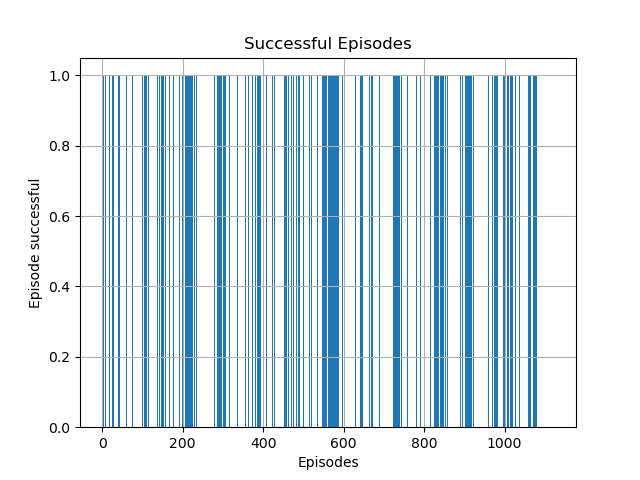
\includegraphics[width=0.7\linewidth]{Images/original_algorithm/successful_episode}
		\caption[Successful episodes]{Evolution of successful episodes during training}
		\label{fig:successfulepisode}
	\end{figure}
	

